\documentclass[10pt,twocolumn]{article}
\usepackage[margin=0.75in]{geometry}                % See geometry.pdf to learn the layout options. There are lots.
\geometry{letterpaper}                   % ... or a4paper or a5paper or ... 
%\geometry{landscape}                % Activate for for rotated page geometry
%\usepackage[parfill]{parskip}    % Activate to begin paragraphs with an empty line rather than an indent
\setlength{\columnsep}{1cm}
\usepackage{graphicx}
\usepackage{amssymb}
\usepackage{epstopdf}
%\usepackage{fullpage}
\usepackage[usenames]{color}
%\usepackage{titlesec}
\usepackage{hyperref}
\usepackage{framed}
%\usepackage[none]{hyphenat}
\hyphenpenalty=1000
\exhyphenpenalty=10000

%\definecolor{light-gray}{gray}{0.45}
%\titleformat{\section}
%{\color{black}\normalfont\huge\bfseries}
%{\color{black}\thesection}{1em}{}

%\titleformat{\subsection}
%{\color{light-gray}\normalfont\Large\bfseries}
%{\color{light-gray}\thesubsection}{1em}{}

%\DeclareGraphicsRule{.tif}{png}{.png}{`convert #1 `dirname #1`/`basename #1 .tif`.png}
\DeclareGraphicsExtensions{.png}

\title{\Large{\bf A Silhouette Edge Lab for Computer Graphics}}
\author{Paul Nixon, Tufts University}
% Activate to display a given date or no date
\date{}

\begin{document}
\maketitle
\begin{figure*}
\centerline{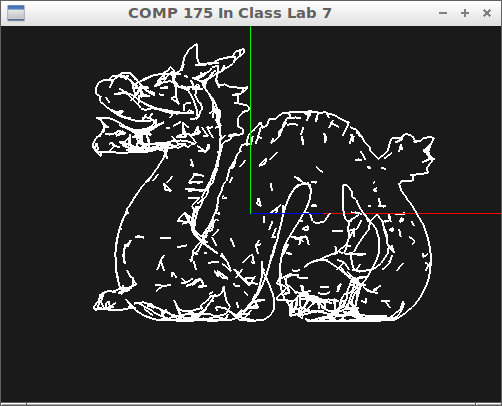
\includegraphics[width=5in]{scrot}}
\caption{Correct Output of a Completed Program}
\end{figure*}

\section{Abstract}
The silhouette edge lab for Tufts's Computer Graphics course was an opportunity for students to learn about non-photorealistic rendering, an important subfield within computer graphics.  They were able to see how the analysis of a basic geometric mesh enabled the discovery of additional properties of the shape.  Additionally, the silhouette edge lab was an opportunity for the instructors to see what choices the students would make when given options for the design of a crucial data structure.  

\section{Background}
In computer graphics, the generation of the silhouette edge is one of the most important fundamental techniques in non-photorealistic rendering.  The silhouette edge appears as the outline of a three-dimensional object or between its parts, but for any viewing angle it can be generated from the usual data required for more common photorealistic rendering techniques.  

The usual representation of an object in computer graphics is to specify a set of three-dimensional points (also called vertices), and then to specify how those points are arranged into triangles.  To draw the triangles, the points are transformed from the three-dimensional space in which they are specified into a two-dimensional space analogous to the screen where they are to be displayed.  From the points which make up each triangle, the normal vector perpendicular to the plane of the triangle is used to simulate the bouncing of light, allowing for photorealistic shading.  

There are many algorithms involved in simulating the physics of how light interacts with objects, but generation of the silhouette edge is not one of them.  In fact, the silhouette edge is defined by the boundary between faces which interact with light at all and those which do not.  

The silhouette edge is made up of those edges on the boundary between faces which can be seen onscreen and faces which are hidden from view.  Its generation is one of the times when computer graphics operates not on faces or on vertices, but on the edges, the places where two faces meet.  

When displayed on its own, it appears as the "outline" of a three-dimensional shape, or the border between parts of the shape.  It is used in situations which require simulation of artists' hand-drawn rendering techniques.  Sometimes this is because an outline can make shapes easier for the viewer to discern, and sometimes this is for purely artistic purposes such as the creation of a "cel-shaded" art style for a video game or movie.  

\section{Motivation}
\subsection{Creation of the Assignment}
The generation of the silhouette edge was chosen for an inclass lab for several reasons.  

First, to expose students to the techniques involved in non-photorealistic rendering.  Second, to have the students work with the geometric principles involved in generation of the silhouette edge.  

\red{Third,  the data structures involved.  }

However, the generation of the silhouette edge was not suitable for inclusion in the out-of-class assignments, because each of those assignments built off the previous one, and focused together on creation of successive techniques in traditional photorealistic rendering.  

\subsection{Occlusion}
There are more steps involved in cel-shading an object from its silhouette edge, but they were deemed infeasible.  A silhouette edge will include edges which on their own have all the properties of the silhouette edge, but would be hidden from view in reality by other parts of the object in between the edge and the viewer.  

To simulate this phenomenon, called occlusion, correctly, each pixel which might be colored as part of the silhouette edge must be checked against each face to see if the face is in the way preventing the pixel from being seen.  To do this in real time is possible, but it requires more advanced techniques than the students had learned at this point in the course.  

\subsection{Simplifications}
To simplify the geometric calculations, an orthographic projection was used.  
To calculate whether a face is facing towards the viewer, it's necessary to know the direction that the viewer is looking into the screen to see that face.  An orthographic projection has the same look vector towards any part of the screen, whereas a perspective projection has different look vectors for each pixel on the screen.  So, to use a perspective projection would have required more geometric calculation.  

To keep the amount of work to a feasible level for students to complete in one hour, some peripheral parts of the program to find and display the silhouette edge were provided to the students.  This included the parser for the mesh files containing faces and vertices, along with a user interface and basic program to load them and display the solid shapes.  This also included the data structures for vertices and faces.  Parsing was considered an important skill, however, and the same parser had in fact been the assignment for a previous lab assignment.  

\section{Problems}
Generation of the silhouette edge can be considered as two related problems: generation of the edge list and the selection of silhouette edge segments.  Of the two, generation of the edge list is more complex.  

\subsection{Edge List Generation}
The list of all edges must be found before the silhouette edge (a subset of the total edge list) can be calculated.  This is a data structure problem involving reading from two structures and creating a third.  

Shapes are specified only as vertices and faces, so generation of the edge list requires iterating through the list of faces and finding all the places where two faces meet (that is, where two points are shared between a pair of faces).  To do this requires understanding of the relation between data and geometry, so that new knowledge can be extracted from the existing data.  It also requires knowledge of the computational representation of data, for there is more than one data structure which can be used to fulfill the requirements of the edge list from which the silhouette edge can be synthesized.  

The vertices, which were read in first from the mesh file, were stored as triples of floating point numbers, as an array by the program in the same order as they were listed in the file.  The triangular faces those vertices were arranged into were read from the file afterwards, stored both in the file and in the program as triples of indices into the vertex list.  

The use of arrays for both the vertex list and the face list made sense because these data structures had a known size indicated by the mesh file header and didn't need to support lookup by anything other than index.  

However, the number of edges isn't necessarily known before the edge list is done being created, and lookup of an edge within the edge list by its constituent vertices is useful during this process.  So an array isn't the best way to store the edge list.  

The set of edges comprising the silhouette edge can change based on the angle at which the shape is being viewed, so the list of all edges must be traversed every time the viewing angle is changed.  The need for speed is a theme in computer graphics programming, and the reason this is an interesting data structures problem is the difference in speed between an adequate data structure and a more optimized one.  

\subsection{Geometric Subproblem}
The geometric aspect of the problem comes afterwards, when the edge list has been created and the silhouette edge is to be found from within it.  This requires calculations for each face based on the face's orientation with respect to the viewer.  Instead of these calculations being used simply to shade each face as in most computer graphics algorithms, they are used for a more drastic choice of whether or not to display an edge at all.  

It is at this stage that the edge list is traversed, checking each pair of adjacent faces to see if the edge between them is a part of the silhouette edge.  

The necessary condition is that one face is facing towards the viewer and the other face is facing away.  This can be detected by calculating the angle between the viewer's look vector and the surface normal vector for each face.  If the angle is less than 90 degrees, the face is towards the viewer and in view, whereas if the angle is 90 degrees or greater, it cannot be seen.  So the algorithm must check this angle for every face.  

In contrast to the overall edge list, the silhouette edge changes every time the viewing angle is changed, hence it is important that it can be calculated quickly.  Conversely, it is not important to store the actual silhouette edge; it can be sent to the graphics hardware and then discarded.  

\subsection{Optimizations}
Some of the values the students were required to calculate could be computed once for each run of the program and stored, instead of calculating them once for every frame.  Since the normal vector for a face does not change, it makes sense to precompute and store this for all faces.  A less obvious optimization is to compute the angle for each face prior to checking the two faces in each edge, since each face is a member of multiple edges.  

\section{Results}
\subsection{Format}
The lab was completed by students in groups of one, two, or three.  There were about ten groups, with one professor and three teaching assistants present.  This allowed the students to work collaboratively and to get help whenever both members of any team got stuck.  

\subsection{Progress}
Most students figured out the algorithm for calculating the edge list within the first half hour of the hour long lab session.  However, the data structure proved to be a point of confusion for several teams.  

When the lab session ended, half of the teams in the room had completed the assignment, and most of the others had either the algorithm or the data structure.  

\subsection{Final Submissions}
When the results were demoed for grading the following week, most groups had completed the assignment successfully, and the one group which had not completely rendered the silhouette edge was able to render most segments of it.  Eight groups sent me their code afterwards (frustratingly, the team with an incomplete silhouette edge was not among them).  

\section{Solutions}
\subsection{Requirements}
Building the edge list was the more difficult part of the problem for most students.  For the data representation of an edge to be useful, each edge must contain some representation of both the vertices contained by the edge (for drawing the edge), and of both the faces containing the edge (for determining if the edge will be drawn).  

The usual approach is to iterate through the list of faces, and for each pair of vertices in a face, either add a new edge to the list of edges, or add a new face to the faces in an existing edge.  The aspect of this which lends itself to more than one approach is the lookup of an edge within the edge list.  

\subsection{Hash Table}
The obvious approach is to use some sort of hash table, but the hashing scheme is less obvious, since an edge is uniquely identified by no one piece of data but by a pair of vertices.  One team debated hashing schemes for a good portion of the lab session, but did not end up using any sort of hash.  

\subsection{Arrays}
A less obvious approach is to simply iterate through the entire edge list every time an edge is searched for.  This is an O($n^2$) algorithm, but its use here can be justified by the realization that the edge list only needs to be built once per object, during the initial load of the object file.  If this approach is chosen, the edge list can be made up of a singly-linked list, giving the advantages of an easily expandable and quickly-iterable data structure.  

However, no teams chose to use linked lists.  Two teams used a standard library vector, and one team built their own expanding array.  These teams had severely increased runtimes for edge list generation, probably due to the cost of allocating a larger array and copying from the old one when the array ran out of space.  However, the silhouette edge was still produced correctly and in approximately the same amount of time.  

\subsection{Hybrid Structure}
My own solution to the data structure problem was to use an edge list made up of an array of linked lists.  The array was the same size as the vertex list and indexed by the lower of the two vertex indices for a given edge.  The linked lists were used because a vertex could have several edges for which it was the lower-numbered vertex.  

This provides a O($k \times n$) algorithm, where $k$ is the maximum number of faces per vertex.  In the worst case, all faces meeting at one point, this is O($n^2$).  

The students were not required to use the same data structure, but the declaration for it was included and some groups chose to use it.  

In retrospect, this was a mistake.  The use of a hybrid data structure was confusing to the students, produced more trouble spots in code, and made even my own solution more difficult to write.  These disadvantages were not outweighed by the advantage of faster edge list creation, and a simple singly-linked list would have been a more sensible solution.  

Among the code I saw, three teams used my hybrid data structure for the edge list.  The final code did not show any signs of the struggles they may have had in using it.  

\subsection{Matrix}
One team had the interesting idea to use a matrix for edge list generation, with each dimension of the array equal to the number of vertices.  Each combination of two different vertices would correspond to two different elements of this matrix, so for each edge appearing in the shape, the two triangles containing the edge could be indicated within the cells of the matrix.  

After iterating through the faces to fill in the matrix, the edge list could be built from one pass through the matrix and the matrix discarded.  This data structure made lookup during edge list generation easy, but at the cost of a vast space requirement.  It worked well for smaller sizes of input but not for larger shapes.  

\subsection{Ordering}
One data structure difference within the individual edges was the choice of whether to maintain an ordering condition of the faces within the edge, or to check each combination when searching for an edge within the edge list.  This was a requirement when using the hybrid data structure as the array was indexed by the lower-numbered edge, but neither the team using the standard library vector nor the team who built their own expandable array decided to maintain this condition.  The result of this was that the extra traversal steps for the hybrid data structure had approximately the same code size as the extra checks for the non-hybrid data structures.  

\subsection{Geometry}
The geometric parts of the algorithm were almost identically similar among different teams' implementations, since the mathematical definition of the silhouette edge did not leave much room for creativity.  All groups used the sign of the dot product (scalar product) instead of the actual angle for deciding if a face was facing towards or away from the viewer, but only a few teams had the idea of multiplying two dot products and checking the sign to check if their signs were opposite.  

\section{Conclusion}
The silhouette edge lab was an opportunity for students to work on an entirely different style of rendering than the style used in the rest of the computer graphics course.  It was a slight departure from the techniques used in the rest of the course, but the students were able to adapt to this and quickly grasp the additional geometric and data structure concepts at work in generation of the silhouette edge.  Although this was the only foray that many of these students had into the realm of non-photorealistic rendering, the silhouette edge lab allowed them to familiarize themselves with one of its central concepts.  

This lab was also an opportunity for students to use a different data structure depending on their personal preference and coding style.  In this, also, the students did not disappoint.  Even though the final result was mathematically constrained, multiple correct solutions were able to be developed.  

\end{document}  